\documentclass[10pt,a4paper]{article}
\usepackage[utf8]{inputenc}
\usepackage{amsmath}
\usepackage{amsfonts}
\usepackage{amssymb}
\usepackage{multicol}
\usepackage{graphicx}
\usepackage{caption}
\usepackage{subcaption}
\begin{document}

\section{2D lid-driven cavity}

\subsection{Case A}

\begin{figure}
\centering
\begin{minipage}{.5\textwidth}
  \centering
  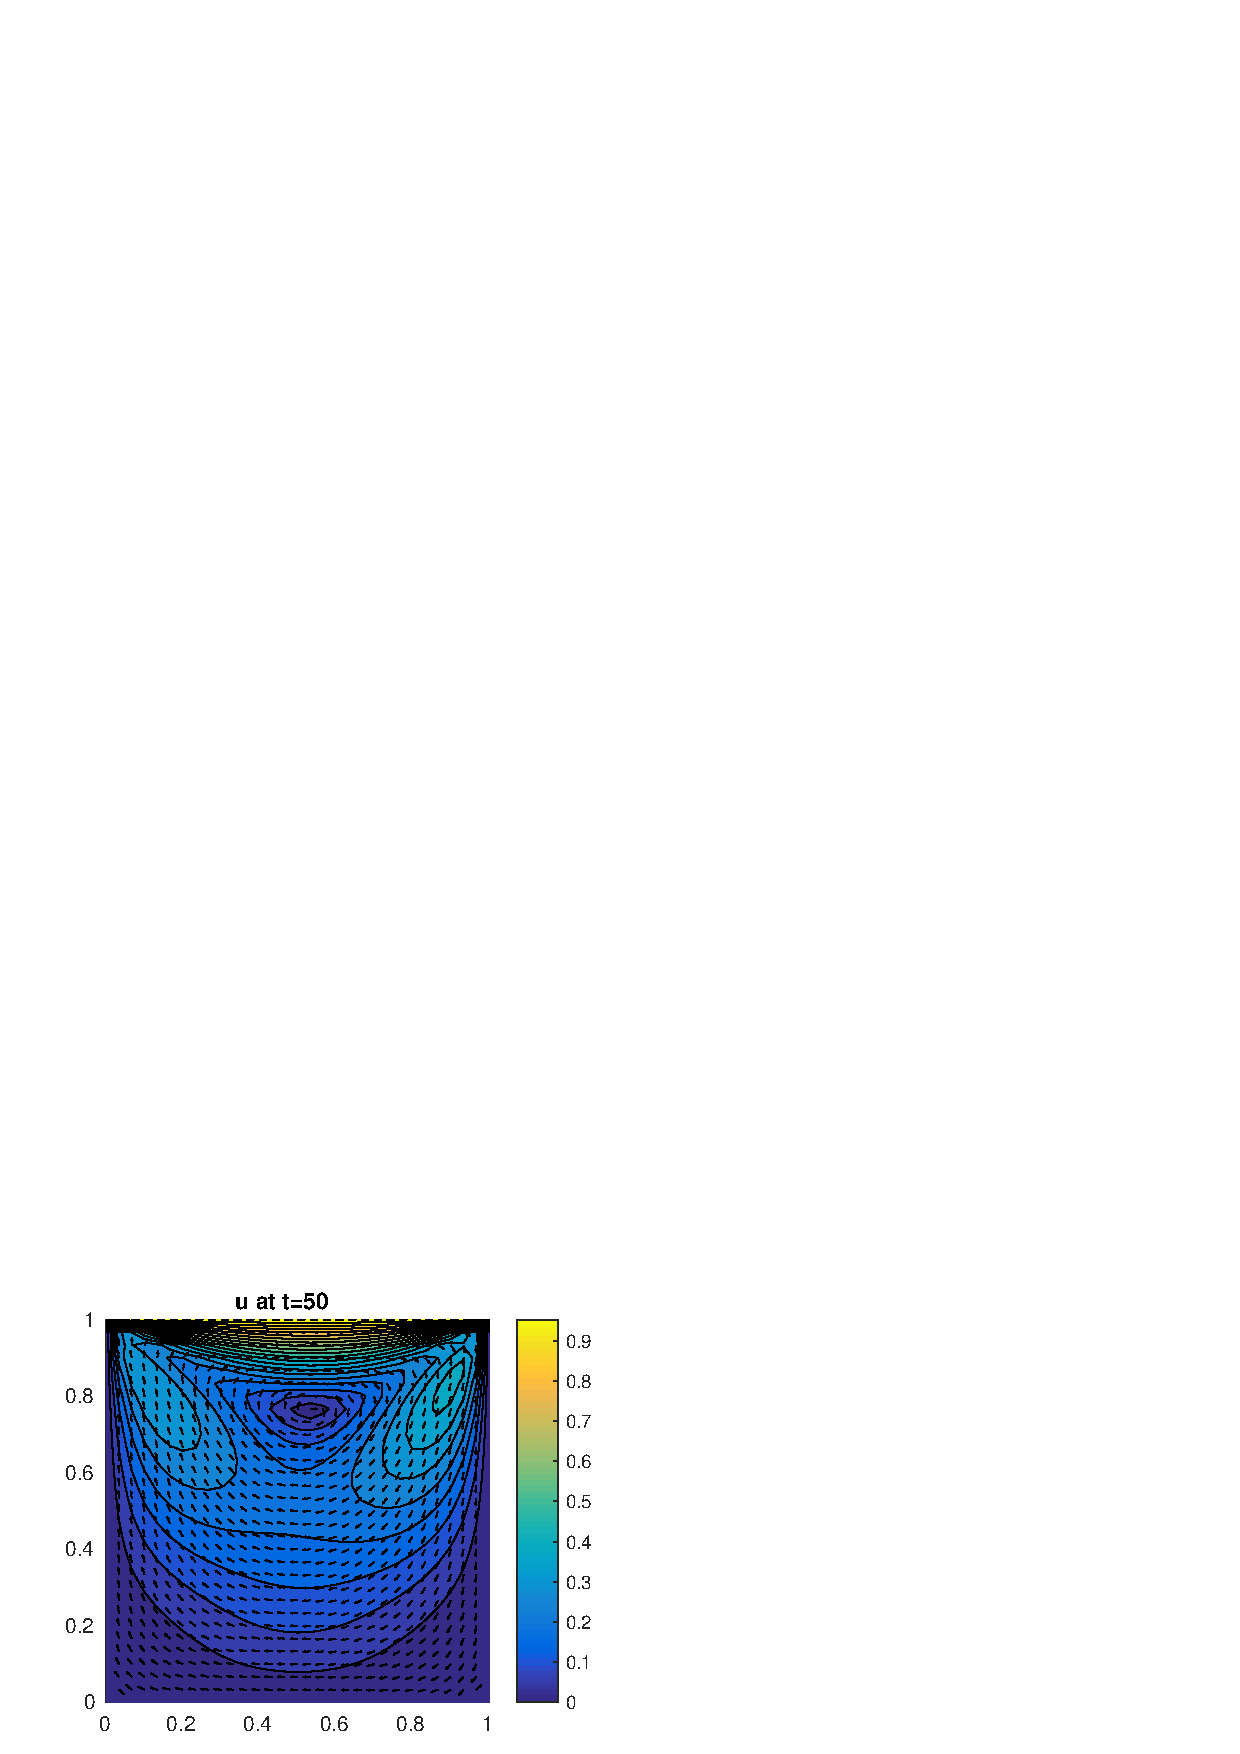
\includegraphics[width=.9\linewidth]{Part1_Case_A_Velocity.pdf}
\end{minipage}%
\begin{minipage}{.5\textwidth}
  \centering
  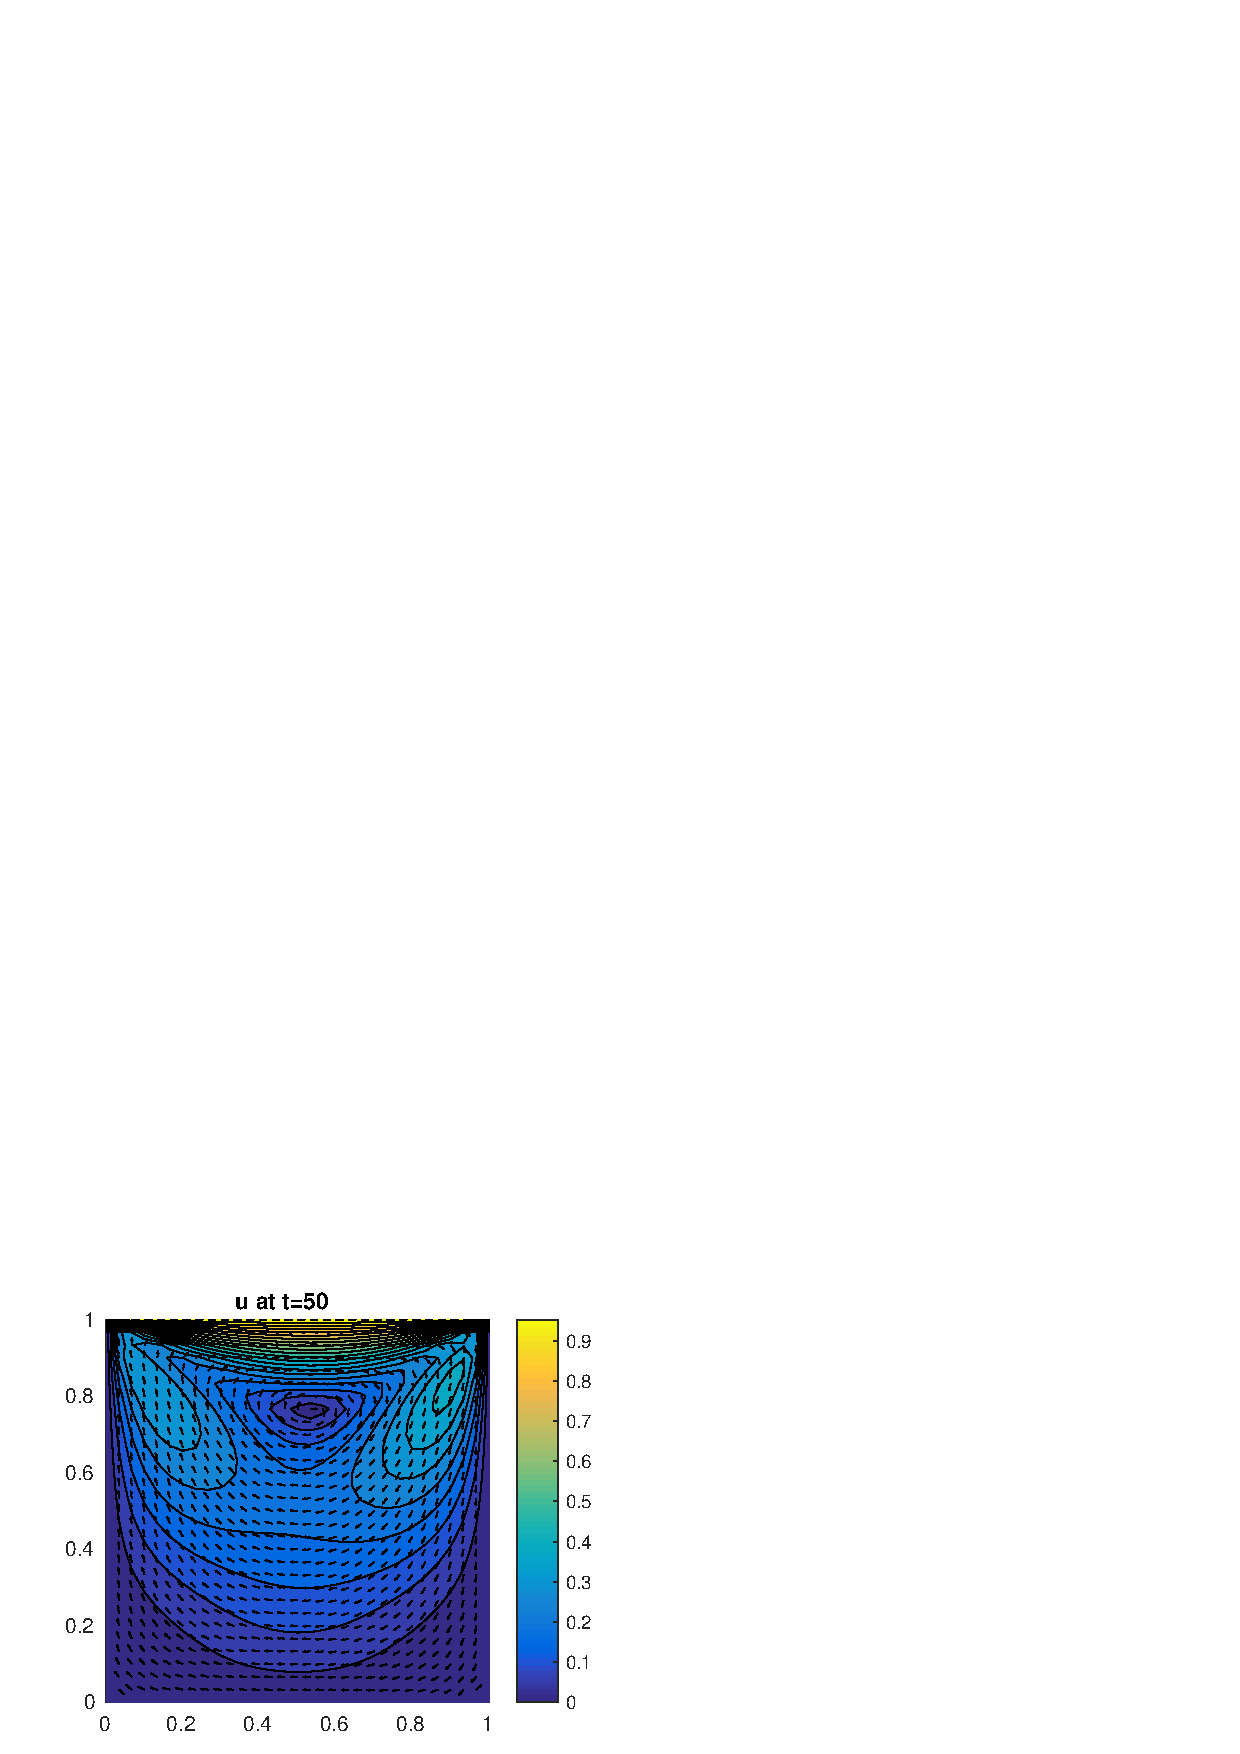
\includegraphics[width=.9\linewidth]{Part1_Case_A_Velocity.pdf}
\end{minipage}
\caption{youo}
\end{figure}


\subsection{Case B}

\subsection{Case C}

\newpage
\subsection{Question 1}
\includegraphics[width=\textwidth]{Q1.jpg}

\newpage
\subsection{Question 2}
The two stability conditions for a general 2D advection diffusion problem are stated in equations (\ref{eq:advec}) and (\ref{eq:dif}) and the combined condition includes equations (\ref{eq:dif}) and (\ref{eq:combined}).

\noindent Note: \textit{These equations were derived in lectures and part of the exam so the derivation has been omitted from this report}.

\begin{equation}
\label{eq:advec}
\text{Advection (CFL):  } \sigma_x + \sigma_y \leq 1 
\end{equation}

\begin{equation}
\label{eq:dif}
\text{Diffusion: } \beta_x + \beta_y \leq \frac{1}{2}
\end{equation}

\begin{equation}
\label{eq:combined}
\text{Combined: } \frac{\sigma_x^2}{\beta_x} + \frac{\sigma_y^2}{\beta_y} \leq 2
\end{equation} 

In the case of the non-linear Navier Stokes equations we take $a_x = \max{|u|}$ and $a_y = \max{|v|}$. Furthermore, by assuming $\Delta x = \Delta y = h$, equations (\ref{eq:advec}) - (\ref{eq:combined}) can be further simplified to equations (\ref{eq:dt_CFL}) - (\ref{eq:dt_combined}). A final conservative assumption to equations  (\ref{eq:dt_CFL}) and (\ref{eq:dt_combined}) is that $ \max{|u|} \approx\max{|v|} < U_{lid} = 1$.

\begin{equation}
\label{eq:dt_CFL}
\text{CFL: } \Delta t \leq \frac{h}{\max(|u|) + \max(|v|)}  \approx \frac{h}{2}
\end{equation}

\begin{equation}
\label{eq:dt_diffusion}
\text{Viscous limit: } \Delta t \leq \frac{h^2}{4} \text{Re}
\end{equation}

\begin{equation}
\label{eq:dt_combined}
\text{Combined: } \Delta t \leq \frac{2}{\text{Re} \left(\max(|u|)^2 + \max(|v|)^2\right)}  \approx \frac{1}{Re}
\end{equation}\\




These conditions have been tabulated for cases A - C below:

\begin{center}


\begin{tabular}{c|cccc|ccc}

 & Re & h & $\max(|u|)$ & $\max(|v|)$ & CFL & Viscous & Combined \\ 
\hline 
Case A  & 20 & $\frac{1}{30}$ & •& • & 0.0167 & 0.0056 & 0.0500 \\ 

Case B  & 200  & $\frac{1}{50}$ & •& • & 0.0100 & 0.0200& 0.0050  \\ 

Case C & 4000 & $\frac{1}{100}$ & •& • & 0.0050 & 0.1000 & 0.0003  \\ 

\end{tabular} 
\end{center}


It can be seen that the energy equation takes a similar form to the momentum equation with the Peclet number replacing the Reynolds number. Hence we can assert the following analogous conditions to equations (\ref{eq:dt_diffusion}) and (\ref{eq:dt_combined}):

\begin{equation}
\text{Viscous: } \Delta t_{energy} \leq \frac{2}{\text{Pe} \left(\max(|u|)^2 + \max(|v|)^2\right)}  \approx \frac{1}{Pe} = \frac{1}{Pr}\Delta t_{momentum}
\end{equation}

\begin{equation}
\label{eq:energy}
\text{Combined: } \Delta t_{energy} \leq \frac{h^2}{4} \text{Pe} = Pr \Delta t_{momentum}
\end{equation}

In the case that $Pr = 0.71 < 1$ then in the viscous limit (equation (\ref{eq:energy}))$\Delta t_{energy} < \Delta t_{momentum}$ is a stricter condition.





\newpage
\subsection{Question 3}
\includegraphics[width=\textwidth]{Q3A.jpg}
\newpage
\noindent \includegraphics[width=\textwidth]{Q3B.jpg}
\newpage



\subsection{Question 4}



\subsection{Question 5}

\end{document}